\documentclass[runningheads]{llncs}

\usepackage[T1]{fontenc}
\usepackage{graphicx}
\usepackage{booktabs}
\usepackage{amsmath}
\usepackage{multirow}
\usepackage{xcolor}
\usepackage{enumitem}
\usepackage{hyperref}
\usepackage{url}
\usepackage{array}

\newcommand{\red}[1]{\textcolor{red}{#1}}
\newcommand{\blue}[1]{\textcolor{blue}{#1}}

\begin{document}

\title{Entity Matching with LLMs at Scale: Accuracy, Cost, and Reasoning Effects}

% \author{Anonymous Author(s)}

% \authorrunning{Anonymous}

% \institute{Anonymous Institution}

\author{
Donghao HUANG\inst{1,2}
%\orcidID{0009-0005-6767-4872} 
\and 
Prasan PAI\inst{2}
%\orcidID{0009-0005-6767-4872} 
\and 
Zhaoxia WANG\inst{1}
%\orcidID{0000-0001-7674-5488}
\thanks{Corresponding author: zxwang@smu.edu.sg}
}
\authorrunning{D. Huang, P. Pai and Z. Wang}
\institute{
School of Computing and Information Systems, Singapore Management University, Singapore, Singapore\\
\email{dh.huang.2023@engd.smu.edu.sg, zxwang@smu.edu.sg}
\and
Research and Development, Mastercard, Arlington, VA, USA\\
\email{donghao.huang@mastercard.com, prasan.pai@mastercard.com}
}

\maketitle

\begin{abstract}
We benchmark large language models for entity matching (EM) using the Compound Entity Matching (ComEM) framework, evaluating 46 model configurations across 8 datasets under a fixed protocol. Beyond accuracy, we quantify \emph{API-equivalent token cost} and analyze the impact of configurable \emph{reasoning/thinking} modes. We find that open-weight models can rival proprietary APIs: GPT-OSS:120b attains 92.10 F1 while costing $\sim$20$\times$ less than GPT-5(high). Reasoning controls have opposite effects across families---low is optimal for GPT-5, whereas high improves open-weight models---and Claude shows the largest sensitivity (Sonnet~4.5: +10.13 F1 with thinking; Opus~4.5: slight degradation at 2.6$\times$ cost). Finally, several ultra-budget configurations under \$0.10 reach up to 89 F1, enabling inexpensive deployment. Our study offers practical model-selection guidance for EM across diverse budget and infrastructure constraints.
\end{abstract}

\keywords{Entity Matching \and Large Language Models \and Entity Resolution \and Open-Weight Models \and Cost-Effectiveness}

\section{Introduction}

Entity matching (EM), the task of determining whether two data records refer to the same real-world entity, is a fundamental step in entity resolution (ER)~\cite{fellegi1969theory,getoor2012entity}. EM has broad applications in data integration, data cleansing, and knowledge graph construction. With the emergence of large language models (LLMs), entity matching has shifted toward zero-shot and few-shot paradigms that eliminate the need for extensive labeled training data~\cite{narayan2022can,peeters2023using,peeters2025entity}.

Wang et al.~\cite{wang2025match} investigated three strategies for LLM-based entity matching---matching, comparing, and selecting---and proposed the Compound Entity Matching (ComEM) framework that composes multiple strategies and LLMs. Their work demonstrated that incorporating record interactions through the selecting strategy yields superior results, and that ComEM achieves both effectiveness and cost-efficiency improvements. However, their evaluation was conducted primarily with GPT-3.5 Turbo and GPT-4o Mini, leaving several important questions unanswered.

First, with the rapid evolution of LLMs, it is unclear how newer model generations---including GPT-4.1, GPT-5, and GPT-5.2---perform on entity matching tasks. Second, open-weight models have made remarkable progress, yet their viability for entity matching within the ComEM framework remains unexplored. Third, modern LLMs offer configurable reasoning effort levels (low, medium, high), and the relationship between reasoning effort and entity matching performance has not been studied. Finally, cost-effectiveness across the current model landscape needs systematic evaluation to provide practical deployment guidance.

In this paper, we address these gaps through a comprehensive empirical study. Our contributions are:

\begin{itemize}[leftmargin=*,itemsep=2pt]
    \item We conduct one of the largest evaluations of LLM-based entity matching to date, testing 46 model configurations across 8 ER benchmark datasets using the ComEM framework, spanning GPT, Claude, and diverse open-weight model families.
    \item We demonstrate that open-weight models now rival proprietary APIs: GPT-OSS:120b achieves 92.10 F1, outperforming all prior-generation proprietary baselines while costing 20$\times$ less than premium models.
    \item We discover that reasoning effort has opposite effects across model families: low reasoning is optimal for GPT-5, high for open-weight models, and Claude models show the most dramatic thinking impact (+10.13 F1 for Sonnet~4.5, yet $-$0.25 for Opus~4.5).
    \item We provide comprehensive cost-performance analysis to guide model selection across diverse budget constraints.
\end{itemize}

\section{Related Work}

\textbf{Entity Resolution and Matching.}
Entity resolution has been studied extensively~\cite{fellegi1969theory,getoor2012entity,papadakis2021blocking,binette2022almost}. The blocking-and-matching pipeline is the dominant approach, where blocking filters out obviously dissimilar records and matching identifies duplicates through various techniques. Traditional methods include rule-based~\cite{benjelloun2009swoosh}, distance-based~\cite{bilenko2003adaptive}, and learning-based approaches~\cite{li2015rule,mudgal2018deep,barlaug2021neural}. More recently, pre-trained language models have advanced entity matching~\cite{li2020deep,tu2023unicorn}.

\noindent\textbf{LLM-Based Entity Matching.}
The advent of LLMs has introduced zero-shot and few-shot paradigms for entity matching~\cite{narayan2022can,peeters2023using,fan2024cost,li2024leveraging,peeters2025entity}. Wang et al.~\cite{wang2025match} conducted a comprehensive investigation of three strategies---matching, comparing, and selecting---and proposed ComEM, which composes strategies and models for improved effectiveness and cost-efficiency. Their work identified that the selecting strategy, which leverages record interactions by presenting all candidates simultaneously, consistently outperforms pairwise matching.

\noindent\textbf{Open-Weight and Reasoning-Enhanced LLMs.}
Recent open-weight models have narrowed the gap with proprietary APIs across many NLP tasks. Models such as DeepSeek~\cite{deepseek2025r1}, Qwen~\cite{qwen2025technical}, and Llama~\cite{dubey2024llama} have demonstrated competitive performance. Additionally, reasoning-enhanced models with configurable thinking effort have emerged as a key trend, with models offering low, medium, and high reasoning settings that trade off computational cost for potential accuracy gains~\cite{fu2025scaling}. However, the impact of these developments on entity matching remains largely unexplored.

\section{Background: ComEM Framework}

\subsection{Problem Formulation}

Following Wang et al.~\cite{wang2025match}, we formulate entity matching as identifying the matching record from a given anchor record $r$ and its $n$ potential matches $R = \{r_1, r_2, \ldots, r_n\}$ obtained from blocking. This formulation accommodates both single-source deduplication and dual-source record linkage under the one-to-one matching assumption.

\subsection{Strategies for LLM-Based Entity Matching}

Three strategies have been proposed for applying LLMs to entity matching:

\textbf{Matching.} The LLM acts as a binary classifier, independently determining whether each pair $(r, r_i)$ is a match. This strategy ignores global consistency among record relationships.

\textbf{Comparing.} The LLM compares two candidate records $r_i$ and $r_j$ against anchor record $r$ to determine which is more consistent. This introduces pairwise record interactions but requires $\mathcal{O}(kn)$ LLM invocations.

\textbf{Selecting.} The LLM directly selects the matching record from the candidate list $R$, leveraging full context of all candidates. This requires only $\mathcal{O}(1)$ LLM invocations per anchor record but is sensitive to position bias in long contexts.

\textbf{ComEM: Compound Entity Matching}
ComEM~\cite{wang2025match} addresses the limitations of individual strategies through a two-stage pipeline: (1)~\emph{Ranking}---a cost-efficient LLM (Flan-T5-XL) scores all $n$ candidates using the matching strategy, retaining the top-$k$ candidates; (2)~\emph{Selection}---a more capable LLM applies the selecting strategy on the filtered $k$ candidates.  The selecting prompt supports a ``[0] if there is none'' option, allowing the model to abstain when no candidate matches. Wang et al.\ show that $k{=}4$ balances F1 and cost, and that this two-stage design mitigates position bias, reduces context length, and improves cost-efficiency.

\section{Experimental Setup}

\subsection{Faithfulness to ComEM Protocol}

To ensure a fair comparison and isolate the effect of model choice as the sole variable, we replicate the ComEM evaluation protocol exactly. Specifically we inherit: (i)~\textbf{Datasets and blocking}: the same 8 pyJedAI~\cite{nikoletos2022jedai} clean-clean ER datasets---spanning product (AB: Abt-Buy, AG: Amazon-Google, WA: Walmart-Amazon), citation (DA: DBLP-ACM, DS: DBLP-Scholar), and entertainment (IM: IMDB-TMDB, IV: IMDB-TVDB, TT: TMDB-TVDB) domains---with Sparkly~\cite{paulsen2023sparkly} blocking at $n{=}10$ candidates; (ii)~\textbf{Sampling}: 400 anchors per dataset (300 with matches, 100 without; random seed 42), yielding 4{,}000 candidate pairs; (iii)~\textbf{Prompts}: the identical matching, comparing, and selecting prompt templates from Wang et al.~\cite{wang2025match} (their Table~5), including the ``[0] if there is none'' abstention option; (iv)~\textbf{ComEM pipeline}: Flan-T5-XL as the ranking model with $k{=}4$ candidates retained for selection; (v)~\textbf{Decoding}: temperature~$=0$ for all models; (vi)~\textbf{Candidate ordering}: blocking-score order, consistent with Wang et al., so any position bias is identical across models.
We do not shuffle candidates because our goal is controlled comparison under the same positional-bias conditions analyzed in ComEM; randomization would introduce an additional variable. The only change is the selecting-stage LLM and, where supported, its reasoning effort or thinking mode; all other pipeline components remain fixed.

% We confirm methodological faithfulness in the Appendix (Table~\ref{tab:per_dataset}): our replication of GPT-4o-Mini achieves 85.9 mean F1 vs.\ Wang et al.'s 86.4---a difference of less than 1\%---validating that our pipeline faithfully reproduces the ComEM protocol.

\subsection{Models Evaluated}

We evaluate an extensive set of 46 model configurations spanning four categories:

\textbf{Proprietary API models (OpenAI):} GPT-4o-mini, GPT-4o, GPT-4.1-nano, GPT-4.1-mini, GPT-4.1, GPT-5-nano (low/medium/high reasoning), GPT-5-mini (low/medium/high), GPT-5 (low/medium/high), GPT-5.2 (low/medium/high).

\textbf{Proprietary API models (Anthropic):} Claude-Haiku-4.5 (with/without thinking), Claude-Sonnet-4.5 (with/without thinking), Claude-Opus-4.5 (with/without thinking), Claude-Sonnet-4.6 (with/without adaptive thinking), Claude-Opus-4.6 (with/without adaptive thinking).

% [R1C1]: R1 Comment 1 — clarify GPT-OSS naming: these are Ollama registry model IDs, not a public model family; identify underlying open-source models (e.g., Qwen2.5-72B for gpt-oss:20b, etc.)
% [R1C2]: R1 Comment 2 — add deployment details: batch size, concurrency settings, and actual inference time on NVIDIA DGX Spark
\textbf{Open-weight models (locally deployed with Ollama):} All model names follow the Ollama community registry naming convention (e.g., \texttt{gpt-oss:20b}), accessible via \texttt{ollama pull gpt-oss:20b}. The names \texttt{gpt-oss:20b} and \texttt{gpt-oss:120b} are Ollama registry identifiers for open-weight model checkpoints; they are not a publicly named model series. This category also includes GLM-4.7-Flash%:q4\_K\_M (4-bit quantized)
, Gemma3:27b, Llama4:Scout, and Granite4:32b. Models are deployed locally on an NVIDIA DGX Spark (128\,GB unified memory) using Ollama v0.15.6 with sequential inference (batch size~$=1$, single concurrent request), and \texttt{num\_ctx=8192}. Typical wall-clock inference latency on DGX Spark was 30--120\,s per anchor for the 120b model and 8--30\,s for the 20b model; we report API-equivalent token cost as a hardware-independent proxy (see Section~\ref{sec:cost}).

\textbf{Open-weight models (via OpenRouter API):} DeepSeek-Chat-v3.1 (with/ without reasoning), Kimi-K2-0905, Kimi-K2-Thinking, GLM-5 (with/without thinking), Qwen3-235b-a22b-2507 (standard and thinking variants), and MiniMax-M2.5. These models are accessed through the OpenRouter API.

% [R1C3]: R1 Comment 3 — supplement with official per-provider definitions of reasoning levels (e.g., OpenAI's low/medium/high budget tokens, Anthropic's thinking budget_tokens, Ollama's think flag); clarify what "high" means in API call parameters for each family
Reasoning effort levels (low, medium, high) or thinking modes (enabled, adaptive, disabled) are configured where supported, enabling systematic study of the reasoning--performance trade-off. These are provider-specific controls with differing internal semantics; we study them as practical deployment knobs rather than a standardized compute measure. Concretely: \textbf{OpenAI GPT-5 family} exposes a \texttt{reasoning\_effort} parameter (\texttt{low}/\texttt{medium}/\texttt{high}) that controls the number of internal reasoning tokens the model generates before output---higher effort incurs greater latency and token cost. \textbf{Anthropic Claude} exposes a \texttt{thinking} parameter (\texttt{enabled}/\texttt{disabled}/\texttt{adaptive}); when enabled, the model produces a hidden extended-thinking block before the visible response, with \texttt{adaptive} letting the model decide whether thinking is beneficial. \textbf{Open-weight models via OpenRouter} (DeepSeek, GLM-5) support a reasoning toggle that activates chain-of-thought tokens; Kimi-K2-Thinking is a separate checkpoint trained for reasoning. \textbf{Locally deployed models} are invoked with Ollama's \texttt{think=true/false} flag. Because internal mechanics differ across providers, cross-family comparisons of effort levels are not meaningful; only within-family comparisons are made.

\subsection{Cost Calculation}
\label{sec:cost}

We report \emph{API-equivalent token cost}, computed from measured token counts and published per-token prices (as of Feb.\ 17, 2026). Proprietary models use their providers' pricing; open-weight models---whether locally deployed or accessed via API---use OpenRouter's published unit pricing as a uniform proxy. This differs from Wang et al.'s~\cite{wang2025match} approach of estimating open-source cost via inference time $\times$ cloud GPU hourly rate; our metric is hardware-independent and comparable \emph{as an API-equivalent proxy} across models. Cost per run is:
\begin{equation}
\text{Cost} = N_{\text{in}} \times P_{\text{in}} + (N_{\text{out}} + N_{\text{reason}}) \times P_{\text{out}},
\label{eq:cost}
\end{equation}
where $N_{\text{in}}$, $N_{\text{out}}$, and $N_{\text{reason}}$ are the numbers of input, output, and reasoning tokens, respectively, and $P_{\text{in}}$ and $P_{\text{out}}$ are the corresponding per-token prices. 
% [R1C6]: R1 Comment 6 — add a worked numerical example immediately after Eq.~\ref{eq:cost} to illustrate the cost calculation (e.g., show sample token counts and prices for one model-dataset pair)
\emph{Example:} for \texttt{gpt-5(low)} on a single anchor with $N_\text{in}{=}500$, $N_\text{out}{=}10$, $N_\text{reason}{=}200$ tokens at OpenAI prices $P_\text{in}{=}\$1.50/\text{M}$, $P_\text{out}{=}\$8.00/\text{M}$: cost $= 500{\times}1.5{\times}10^{-6} + (10{+}200){\times}8.0{\times}10^{-6} = \$0.00075 + \$0.00168 = \$0.00243$ per anchor; summed over 3,200 anchors, total $\approx\$7.78$, broadly consistent with the \$6.25 reported for \texttt{gpt-5(low)} in Table~\ref{tab:compound_performance} (the difference reflects actual vs.\ illustrative token counts).

% [R1C7]: R1 Comment 7 — clarify rationale for using total (summed) cost across all 8 datasets rather than per-dataset average; add a sentence explaining the design choice
For locally deployed models, we report API-equivalent token cost as a hardware-independent proxy; actual on-prem cost depends on amortization, utilization, and power. All costs in this paper are \emph{summed} across 8 datasets (3{,}200 anchors total). We chose summation over per-dataset averaging primarily for numerical precision: several budget models cost only a few cents per dataset, making per-dataset figures indistinguishable at two decimal places---for example, GPT-4.1-mini and GPT-5-nano(low) (\$0.26 and \$0.29 total, respectively; Table~\ref{tab:full_ranking}) would both round to \$0.03 per dataset, obscuring a meaningful 12\% cost difference. To obtain per-dataset cost, divide by 8. Wang et al.~\cite{wang2025match} report per-dataset cost, so our totals are exactly $8\times$ larger for comparable models---for example, our GPT-4o-Mini total of \$0.72 corresponds to their reported \$0.09 per dataset.

% \subsection{Response Parsing}

% The selecting prompt asks the LLM to return a bracketed index (e.g., \texttt{[1]} or \texttt{[0]} for no match). We extract the index using the regex \texttt{\textbackslash[(\textbackslash d+)\textbackslash]}; unparseable responses (e.g., verbose preamble, refusal, empty output) default to \emph{no match}, penalizing recall rather than inflating match predictions. We apply the same parser and fallback rule to all models. We verified parse-failure rates by scanning all cached responses (Appendix, Table~\ref{tab:invalid_rate}): 28 of 46 models achieve 0\%. Notable outliers include GPT-5-nano(high) at 30.6\%---likely contributing to its anomalously low F1 despite high precision---and GLM-5 at 11--20\%. All Claude~4.6 configurations achieve 0\%, suggesting that thinking modes do not degrade format compliance. For GPT-5, the invalid rate rises from 0\% (low) to 0.3\% (medium) to 5.8\% (high), indicating that higher reasoning effort can increase verbosity-related failures; we therefore report invalid response rates to contextualize performance under different verbosity regimes.

% % [R1C5]: R1 Comment 5 — add qualitative analysis or example responses showing why GPT-5-nano(high) high reasoning leads to format violations (verbosity, preamble, refusals); include 1-2 actual response examples in appendix or inline
% % [R1C5]: VERIFIED 2026-03-20 via notebooks/gpt5_nano_high_invalid_analysis.ipynb — all 978 invalid responses confirmed as reasoning token exhaustion (empty content, finish_reason=length, reasoning_tokens=2048).
% Inspection of all 978 invalid responses from GPT-5-nano(high) reveals a single failure mode: \textbf{reasoning token exhaustion}. In every case the model's internal chain-of-thought consumes all 2{,}048 allowed completion tokens (\texttt{reasoning\_tokens\,\\=\,completion\_tokens\,=\,2048}), triggering a \texttt{length} finish and leaving zero tokens for visible output. The response content is an empty string---the model never produces the required bracketed index because it never produces any output at all. By contrast, GPT-5-nano(low) completes reasoning within budget for all 3{,}200 queries (0\% invalid), using an average of only 185 reasoning tokens per response. GPT-5-nano(medium) shows an intermediate pattern: 3.7\% of responses exhaust the budget at an average of 643 reasoning tokens. This progression---185 (low, 0\%), 643 (medium, 3.7\%), 1{,}111 (high, 30.6\%)---demonstrates that higher reasoning effort in nano-class models triggers disproportionately deep deliberation that exceeds the token budget, a problem less severe in larger models where GPT-5(high) reaches only 5.8\% at 650 average reasoning tokens.

% [R1C7]: R1 Comment 7 (also here) — this is where total cost metric is defined; cross-reference with §4.4 rationale for sum vs. average
\subsection{Evaluation Metrics}

We evaluate all models using the compound strategy, which demonstrated the best overall performance in prior work~\cite{wang2025match}. We report F1 score on the positive class (matching pairs) and total API-equivalent token cost across all 8 datasets (see Section~\ref{sec:cost} for cost definition and rationale for using summed rather than per-dataset cost).

\section{Results and Discussion}

\subsection{Overall Model Performance with Compound Strategy}

% [R1C8]: R1 Comment 8 — add a sentence here calling out that Table~\ref{tab:per_dataset} validates replication (our GPT-4o-Mini 85.9 ≈ original 86.4); make this validation more prominent
Before reporting new results, we note that our replication of GPT-4o-Mini achieves 85.9 mean F1 vs.\ Wang et al.'s 86.4 (Table~\ref{tab:per_dataset}, Appendix), a difference of $<$1\%. Cost is also consistent: our total of \$0.72 equals exactly $8\times$ their reported \$0.09 per dataset, confirming that both outputs and token usage faithfully reproduce the ComEM protocol. All new results below are therefore directly comparable to the ComEM baseline.

Table~\ref{tab:compound_performance} presents the top 15 models alongside selected baselines. GPT-5 and GPT-5.2 variants hold the top 6 positions (93.17--92.14 F1). GPT-OSS:120b(high) ranks 7th (92.10) as the top open-weight model, and Kimi-K2-Thinking ranks 8th (91.84) as the best non-GPT model. All top-15 models exceed 91 F1, with Claude-Haiku-4.5(think) at rank 15 (91.19) as the best Claude configuration.

% [R1C4]: R1 Comment 4 — improve Table 1 readability: add grouping lines between GPT-5 family / open-weight / Claude groups, or split into sub-tables; consider using \midrule between model families
\begin{table}[!ht]
\centering
\caption{Top 15 of 46 model configurations (compound strategy)%, ranked by mean F1 across 8 datasets
. Row numbers (\#) indicate global rank; the full ranking appears in Table~\ref{tab:full_ranking} (Appendix). Cost = total API-equivalent token cost summed over all 8 datasets% (divide by 8 for per-dataset cost)
. Models are grouped by family%; GPT-5-mini is proprietary but ranked 9--11 by F1
.}
\label{tab:compound_performance}
\small
\setlength{\tabcolsep}{3pt}
\begin{tabular}{rlcccc}
\toprule
\textbf{\#} & \textbf{Model} & \textbf{F1} & \textbf{Prec.} & \textbf{Recall} & \textbf{Cost} \\
\midrule
\multicolumn{6}{l}{\emph{GPT-5 / GPT-5.2 family (proprietary API)}} \\
\midrule
1 & gpt-5(medium) & 93.17$\pm$6.0 & 92.04 & 94.42 & \$12.29 \\
2 & gpt-5(low) & 93.14$\pm$6.4 & 92.26 & 94.12 & \$6.25 \\
3 & gpt-5.2(low) & 92.75$\pm$5.9 & 90.58 & 95.12 & \$3.43 \\
4 & gpt-5.2(high) & 92.54$\pm$6.1 & 90.22 & 95.08 & \$5.74 \\
5 & gpt-5.2(medium) & 92.53$\pm$6.2 & 90.33 & 94.92 & \$4.52 \\
6 & gpt-5(high) & 92.14$\pm$6.8 & 92.66 & 91.71 & \$24.50 \\
9 & gpt-5-mini(low) & 91.72$\pm$6.1 & 88.64 & 95.08 & \$0.71 \\
10 & gpt-5-mini(high) & 91.62$\pm$6.2 & 88.47 & 95.08 & \$2.30 \\
11 & gpt-5-mini(medium) & 91.46$\pm$6.4 & 88.21 & 95.04 & \$1.28 \\
\midrule
\multicolumn{6}{l}{\emph{Open-weight models (Ollama / OpenRouter)}} \\
\midrule
7 & gpt-oss:120b(high) & 92.10$\pm$6.3 & 89.91 & 94.46 & \$1.20 \\
8 & kimi-k2-think & 91.84$\pm$6.4 & 90.00 & 93.83 & \$8.29 \\
12 & gpt-oss:20b(high) & 91.36$\pm$6.5 & 89.86 & 93.00 & \$0.46 \\
13 & minimax-m2.5 & 91.34$\pm$5.7 & 90.64 & 92.12 & \$3.74 \\
14 & gpt-oss:120b(medium) & 91.26$\pm$7.2 & 90.29 & 92.33 & \$0.38 \\
\midrule
\multicolumn{6}{l}{\emph{Claude family (proprietary API)}} \\
\midrule
15 & claude-haiku-4.5(think) & 91.19$\pm$6.4 & 88.63 & 94.00 & \$8.64 \\
% \midrule
% \multicolumn{6}{l}{\emph{Selected baselines and notable models}} \\
% \midrule
% 20 & claude-opus-4.6(adapt) & 90.13$\pm$6.4 & 86.13 & 94.62 & \$19.05 \\
% 23 & claude-sonnet-4.5(think) & 89.70$\pm$6.4 & 85.23 & 94.79 & \$22.32 \\
% 24 & gpt-4o & 89.58$\pm$6.1 & 89.43 & 89.87 & \$3.10 \\
% 31 & gpt-4o-mini & 85.88$\pm$6.7 & 84.82 & 87.63 & \$0.72 \\
% 40 & claude-opus-4.5 & 80.53$\pm$6.5 & 71.55 & 92.13 & \$22.32 \\
% 41 & claude-opus-4.5(think) & 80.28$\pm$6.9 & 71.19 & 92.08 & \$57.07 \\
% 44 & claude-sonnet-4.5 & 79.57$\pm$6.4 & 70.01 & 92.17 & \$11.92 \\
% 46 & granite4:32b & 78.49$\pm$9.5 & 81.89 & 77.08 & \$0.09 \\
\bottomrule
\end{tabular}
\end{table}

\subsection{Open-Weight Models Match Proprietary Performance}

A central finding of our study is that open-weight models deployed locally now compete with, and in many cases exceed, the performance of prior-generation proprietary models (Table~\ref{tab:compound_performance}).

% [R3C3]: R3 Comment 3 — add 2-3 sentences analyzing WHY open-weight models approach proprietary performance (e.g., model architecture maturity, RLHF training data quality, instruction-following ability, or local inference benefits); provide theoretical/empirical grounding beyond the observation
\textbf{GPT-OSS models.} The \texttt{gpt-oss:120b(high)} model achieves 92.10 F1, ranking 7th overall and outperforming prior-generation proprietary baselines including GPT-4.1 (90.36 F1) and GPT-4o (89.58 F1). At \$1.20 total cost, it costs 20$\times$ less than GPT-5(high) (\$24.50) while delivering 99.96\% of its performance. The smaller \texttt{gpt-oss:20b(high)} achieves 91.36 F1 at only \$0.46---outperforming GPT-4.1 while costing 2.8$\times$ less.

\textbf{Kimi-K2-Thinking.} From Moonshot AI, \texttt{kimi-k2-thinking} achieves 91.84 F1, ranking 8th overall and entering the top 10 as the best non-GPT model. It delivers balanced high performance (90.00 precision, 93.83 recall) at \$8.29 total cost, outperforming all GPT-5-mini variants.

\textbf{MiniMax-M2.5.} MiniMax-M2.5 achieves 91.34 F1, ranking 13th with well-balanced precision (90.64) and recall (92.12) at \$3.74 total cost---competitive with GPT-OSS:120b(medium) and GPT-4.1-mini.

\textbf{Why open-weight models approach proprietary performance.} Several factors explain this convergence. First, \emph{architectural maturity}: recent open-weight model families have adopted training pipelines---including large-scale instruction tuning and RLHF---that closely mirror those of proprietary APIs, substantially narrowing the capability gap on structured reasoning tasks~\cite{dubey2024llama,qwen2025technical}. Second, \emph{task suitability}: entity matching via the ComEM selecting strategy requires structured reasoning over a short, fixed-length candidate list---a well-constrained task that favors models with strong instruction-following, rather than broad world knowledge or creative generation where proprietary models retain larger advantages. Third, \emph{deployment characteristics}: local inference via Ollama eliminates network latency and API throttling, enabling consistent, unconstrained inference.
% ; however, quantization (e.g., Q4\_K\_M for GLM-4.7-Flash) may slightly reduce accuracy relative to full-precision APIs, partially explaining any residual gap.

\subsection{Reasoning Effort: Opposite Effects Across Families}

A surprising finding is that reasoning effort has opposite effects on different model families. Table~\ref{tab:reasoning_effort} summarizes the impact across six model families.

% [R3C2]: R3 Comment 2 — add a ``$\Delta$ Cost'' column to Table~\ref{tab:reasoning_effort} showing the cost change rate between reasoning settings (e.g., cost ratio High/Low), to visually align the cost-performance dimension with the paper's core research theme
\begin{table}[htbp]
\centering
\caption{Impact of reasoning effort across model families. F1 reported as mean across 8 datasets. ``Best'' = recommended setting considering both F1 and cost; $^\ast$medium is marginally higher (93.17 vs.\ 93.14) but costs 2$\times$ more. $\Delta$F1 = F1 range (max$-$min); $\Delta$Cost = cost multiplier from lowest to highest setting. For models with thinking toggle, ``On'' and ``Off'' denote thinking enabled/disabled; ``Adapt'' denotes adaptive thinking.}
\label{tab:reasoning_effort}
\small
\setlength{\tabcolsep}{3pt}
\begin{tabular}{lccccccc}
\toprule
\textbf{Model Family} & \textbf{Low} & \textbf{Medium} & \textbf{High} & \textbf{Best} & \textbf{$\Delta$F1} & \textbf{$\Delta$Cost} & \textbf{Trend} \\
\midrule
gpt-5        & \textbf{93.14} & 93.17 & 92.14 & Low$^\ast$  & 1.03 & 3.9$\times$ & $\downarrow$ \\
gpt-5.2      & \textbf{92.75} & 92.53 & 92.54 & Low  & 0.22 & 1.7$\times$ & $\approx$ \\
gpt-5-mini   & \textbf{91.72} & 91.46 & 91.62 & Low  & 0.26 & 3.2$\times$ & $\approx$ \\
gpt-5-nano   & 88.38 & \textbf{89.34} & 85.71 & Medium  & 3.63 & 6.3$\times$ & $\cap$ \\
gpt-oss:120b & 90.11 & 91.26 & \textbf{92.10} & High & 1.99 & 7.1$\times$ & $\uparrow$ \\
gpt-oss:20b  & 88.74 & 90.87 & \textbf{91.36} & High & 2.62 & 5.8$\times$ & $\uparrow$ \\
\midrule
 & \textbf{Off} & \multicolumn{2}{c}{\textbf{On/Adapt}} & & & & \\
\cmidrule(lr){2-2} \cmidrule(lr){3-4}
claude-sonnet-4.5 & 79.57 & \multicolumn{2}{c}{\textbf{89.70}} & On & 10.13 & 1.9$\times$ & $\uparrow\uparrow$ \\
claude-haiku-4.5  & 82.64 & \multicolumn{2}{c}{\textbf{91.19}} & On & 8.55 & 2.0$\times$ & $\uparrow\uparrow$ \\
claude-opus-4.6   & 85.18 & \multicolumn{2}{c}{\textbf{90.13}} & Adapt & 4.95 & 1.4$\times$ & $\uparrow$ \\
claude-sonnet-4.6 & 82.48 & \multicolumn{2}{c}{82.55} & Adapt & 0.07 & 1.0$\times$ & $\approx$ \\
claude-opus-4.5   & \textbf{80.53} & \multicolumn{2}{c}{80.28} & Off & 0.25 & 2.6$\times$ & $\downarrow$ \\
glm-5        & 79.77 & \multicolumn{2}{c}{\textbf{91.02}} & On & 11.25 & 23$\times$ & $\uparrow\uparrow$ \\
qwen3-235b   & \textbf{86.85} & \multicolumn{2}{c}{81.76} & Off & 5.09 & 34$\times$ & $\downarrow$ \\
deepseek-v3.1 & 79.16 & \multicolumn{2}{c}{\textbf{86.52}} & On & 7.36 & 7.0$\times$ & $\uparrow$ \\
\bottomrule
\end{tabular}
\end{table}

\textbf{GPT-5 family: low reasoning is optimal.} For GPT-5, low reasoning achieves 93.14 F1 at \$6.25, virtually identical to medium (93.17 F1 at \$12.29) while costing 49\% less. High reasoning (92.14 F1 at \$24.50) actually degrades performance while costing 4$\times$ more. This pattern holds for GPT-5-mini, where low (91.72 F1 at \$0.71) outperforms medium (91.46 F1 at \$1.28) at 45\% lower cost.

\textbf{GPT-5.2 family: reasoning effort has minimal impact.} All three reasoning levels achieve nearly identical F1 ($\sim$92.5), with low being the clear value choice at \$3.43 versus \$5.74 for high.

\textbf{Open-weight models: high reasoning is critical.} In stark contrast, GPT-OSS models show dramatic improvement with higher reasoning effort. For \texttt{gpt-oss:120b}, F1 increases from 90.11 (low) to 91.26 (medium) to 92.10 (high)---a 1.99 point range. For \texttt{gpt-oss:20b}, the range is even larger at 2.62 points. This suggests that open-weight models benefit more from extended reasoning, possibly because they have less internalized knowledge about entity matching patterns and rely more on explicit reasoning.

\textbf{Claude models: dramatic and asymmetric thinking effects.} The Anthropic Claude family exhibits the most extreme thinking impacts of any family tested. Thinking primarily boosts precision while maintaining recall: Sonnet~4.5 gains +10.13 F1 (precision +15.22), Haiku~4.5 gains +8.55, and Opus~4.6 gains +4.95 with adaptive thinking.  Yet Opus~4.5 \emph{loses} 0.25 F1 with thinking at 2.6$\times$ cost (\$57.07), and Sonnet~4.6 gains only +0.07.  Without thinking, all Claude models share high recall (92--93\%) but poor precision (70--79\%), suggesting they default to predicting ``match'' without deeper analysis.

\textbf{Thinking can hurt.} Qwen3-235b drops 5.09 F1 with thinking at 34$\times$ cost. GLM-5 with thinking achieves 91.02 F1 (vs.\ 79.77 without), though it remains expensive compared to GLM-4.7-Flash (90.08 F1 at \$1.74). DeepSeek-v3.1 gains +7.36 F1 with reasoning, confirming model-dependent effects.

\subsection{Cost-Performance Analysis}

% [R1C4]: R1 Comment 4 — enlarge Pareto frontier marker size in Figure~\ref{fig:pareto} and use more distinct colors/shapes to improve readability; consider increasing DPI or using a larger figure width
% TODO: redraw Fig. 1 @Prasan
Figure~\ref{fig:pareto} visualizes the cost--F1 trade-off on a log-scaled cost axis. The Pareto frontier comprises 13 of 46 configurations and is dominated by the GPT ecosystem: six GPT-OSS variants (spanning low to high reasoning at both 20b and 120b scales), GPT-5-mini(low), GPT-5.2(low), and GPT-5 at low and medium reasoning. GPT-4.1-nano also appears at the ultra-budget end alongside Gemma3:27b and Qwen3-235b---the only two non-GPT frontier models. No Claude, GLM, or other model family reaches the frontier. The frontier reveals a steep initial slope---moving from \$0.08 to \$1.20 lifts F1 from 84--89 to 92---followed by sharply diminishing returns beyond \$3.

\begin{figure}[!htbp]
\centering
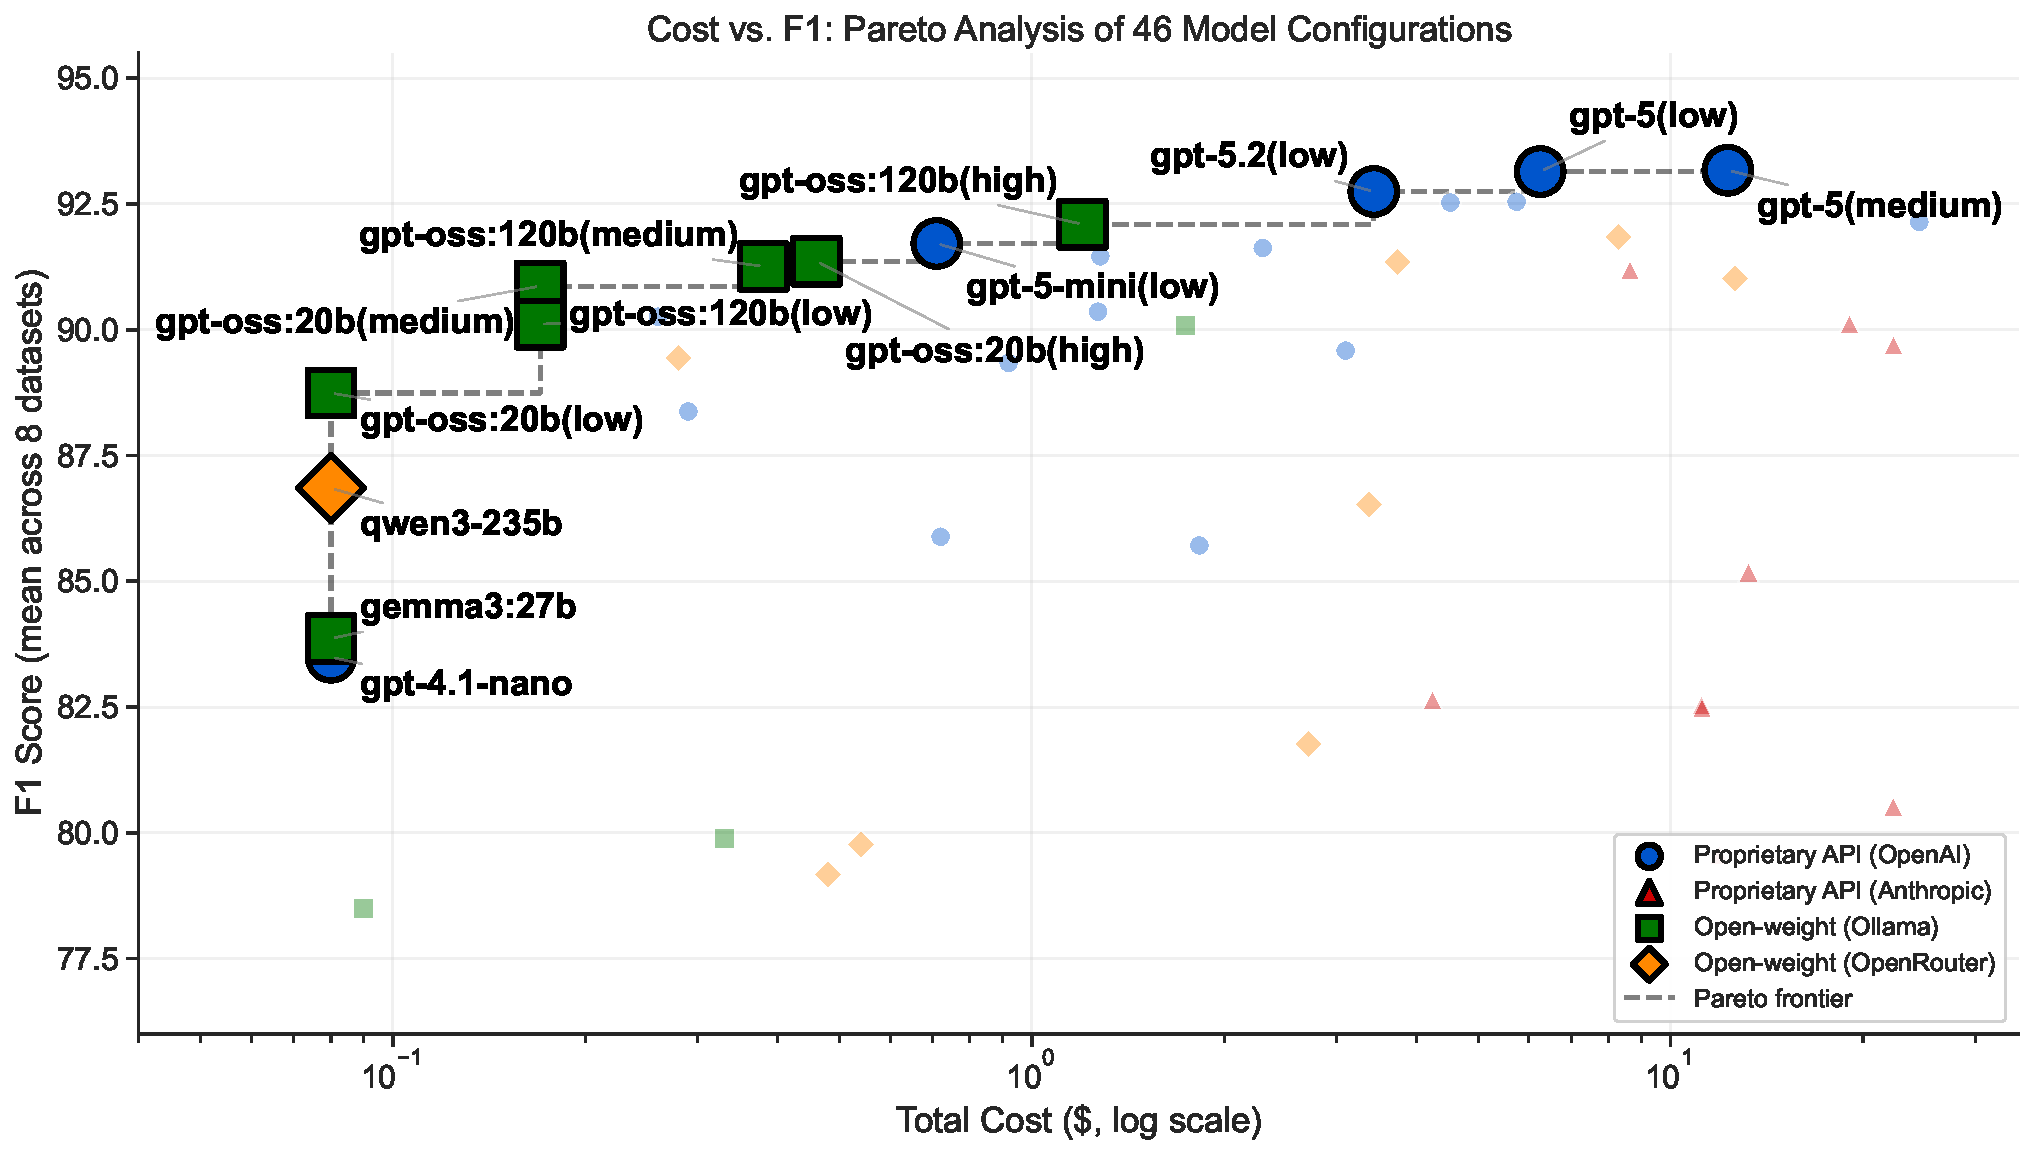
\includegraphics[width=\textwidth]
{pareto_cost_f1_v2.pdf}
\caption{Cost vs.\ F1 Pareto analysis of 46 model configurations using the compound strategy. Each point represents a model's mean F1 (across 8 datasets) and total API cost. The dashed red step line traces the frontier. Marker shapes distinguish proprietary API models (circles), open-weight models deployed locally with Ollama (squares), and open-weight models accessed via the OpenRouter API (diamonds).}
\label{fig:pareto}
\end{figure}

\begin{table}[!htbp]
\centering
\caption{Recommended models by budget tier for entity matching deployment.}
\label{tab:cost_tiers}
\small
\begin{tabular}{lccl}
\toprule
\textbf{Budget Tier} & \textbf{Model} & \textbf{F1} & \textbf{Cost} \\
\midrule
Ultra-budget & qwen3-235b        & 86.85 & \$0.08 \\
Ultra-budget & gpt-oss:20b(low)  & 88.74 & \$0.08 \\
Budget       & gpt-oss:20b(high) & 91.36 & \$0.46 \\
Value        & gpt-5-mini(low)   & 91.72 & \$0.71 \\
Value        & gpt-oss:120b(h)   & 92.10 & \$1.20 \\
Mid-range    & gpt-5.2(low)      & 92.75 & \$3.43 \\
Premium      & gpt-5(low)        & 93.14 & \$6.25 \\
Premium      & gpt-5(medium)     & 93.17 & \$12.29 \\
\bottomrule
\end{tabular}
\end{table}

Table~\ref{tab:cost_tiers} distills these trade-offs into actionable budget tiers. The ultra-budget tier ($<$\$0.10) already achieves 87--89 F1; the budget-to-value range (\$0.46--\$1.20) jumps to 91--92 F1; and beyond \$3 each additional dollar buys less than 0.3 F1 points, making the mid-range and premium tiers worthwhile only when maximum accuracy is critical.

\section{Conclusion}

We present one of the largest empirical evaluations of LLM-based entity matching to date, testing 46 model configurations across 8 benchmark datasets. Open-weight models now rival proprietary APIs at dramatically lower costs (GPT-OSS:120b(high): 92.10 F1 at 20$\times$ less cost). Reasoning effort has opposite effects across families: low is optimal for GPT-5, high for open-weight models, and Claude models show the most dramatic thinking impact (+10.13 F1 for Sonnet~4.5, yet $-$0.25 for Opus~4.5). Several ultra-budget models under \$0.10 achieve up to 89 F1, democratizing entity matching.

% [R3C1]: R3 Comment 1 — expand dirty-data discussion: add qualitative analysis in conclusion or supplementary on how noise/missing values would affect LLM-based EM; or include brief preliminary experimental results on a small dirty dataset
Our study uses clean-clean ER scenarios; performance on dirty data remains to be evaluated. In dirty-data settings---where records contain noise, typos, missing fields, or inconsistent formatting---LLM-based matchers may behave differently from clean-clean benchmarks. Reasoning-enhanced models may prove more robust to noise through extended deliberation that reconciles inconsistent attributes, while smaller or less instruction-tuned models may fail silently by hallucinating attribute values. The ComEM selecting strategy's global view of all candidates simultaneously may help handle missing-field ambiguity better than pairwise matching, since the model can use relative evidence across candidates. Evaluating dirty-data robustness (e.g., on Magellan benchmark dirty datasets~\cite{mudgal2018deep}) is an immediate priority for future work. We inherit the ComEM evaluation protocol, which may not reflect all deployment conditions. Model costs change rapidly, so specific comparisons are illustrative. Future work includes dirty-data evaluation, prompt engineering for open-weight models, adaptive reasoning effort selection, and domain-specific entity matching applications.

% [R1C9]: R1 Comment 9 — standardize reference formatting in references.bib: abbreviate or consistently format conference names (e.g., [23] and similar entries should use uniform abbreviation style per splncs04 conventions)
\bibliographystyle{splncs04}
\bibliography{references}

\appendix

\section{Supplementary Results}
\label{sec:full_ranking}

Table~\ref{tab:full_ranking} presents the complete ranking of all 46 model configurations.

\begin{table}[htbp]
\centering
\caption{Full compound strategy ranking (46 models). F1 = mean$\pm$std across 8 datasets; P/R are means; std omitted for space. Cost = total API-equivalent token cost. Claude models marked $\dagger$. (t)=thinking enabled; (a)=adaptive thinking; (l)/(m)/(h)=low/medium/high reasoning effort.}
\label{tab:full_ranking}
\setlength{\tabcolsep}{1.5pt}
\tiny
\begin{tabular}{rlcrrc|rlcrrc}
\toprule
\textbf{\#} & \textbf{Model} & \textbf{F1} & \textbf{P} & \textbf{R} & \textbf{\$} & \textbf{\#} & \textbf{Model} & \textbf{F1} & \textbf{P} & \textbf{R} & \textbf{\$} \\
\midrule
1 & gpt-5(m) & 93.17\tiny$\pm$6.0 & 92.04 & 94.42 & 12.29 & 24 & gpt-4o & 89.58\tiny$\pm$6.1 & 89.43 & 89.87 & 3.10 \\
2 & gpt-5(l) & 93.14\tiny$\pm$6.4 & 92.26 & 94.12 & 6.25 & 25 & kimi-k2-0905 & 89.43\tiny$\pm$6.0 & 85.25 & 94.21 & 0.28 \\
3 & gpt-5.2(l) & 92.75\tiny$\pm$5.9 & 90.58 & 95.12 & 3.43 & 26 & gpt-5-nano(m) & 89.34\tiny$\pm$6.2 & 84.86 & 94.42 & 0.92 \\
4 & gpt-5.2(h) & 92.54\tiny$\pm$6.1 & 90.22 & 95.08 & 5.74 & 27 & gpt-oss:20b(l) & 88.74\tiny$\pm$7.7 & 88.56 & 89.04 & 0.08 \\
5 & gpt-5.2(m) & 92.53\tiny$\pm$6.2 & 90.33 & 94.92 & 4.52 & 28 & gpt-5-nano(l) & 88.38\tiny$\pm$7.1 & 83.63 & 93.83 & 0.29 \\
6 & gpt-5(h) & 92.14\tiny$\pm$6.8 & 92.66 & 91.71 & 24.50 & 29 & qwen3-235b & 86.85\tiny$\pm$6.3 & 80.54 & 94.54 & 0.08 \\
7 & gpt-oss:120b(h) & 92.10\tiny$\pm$6.3 & 89.91 & 94.46 & 1.20 & 30 & deepseek-v3.1(t) & 86.52\tiny$\pm$8.2 & 88.68 & 84.83 & 3.37 \\
8 & kimi-k2-think & 91.84\tiny$\pm$6.4 & 90.00 & 93.83 & 8.29 & 31 & gpt-4o-mini & 85.88\tiny$\pm$6.7 & 84.82 & 87.63 & 0.72 \\
9 & gpt-5-mini(l) & 91.72\tiny$\pm$6.1 & 88.64 & 95.08 & 0.71 & 32 & gpt-5-nano(h) & 85.71\tiny$\pm$6.0 & 92.61 & 79.92 & 1.83 \\
10 & gpt-5-mini(h) & 91.62\tiny$\pm$6.2 & 88.47 & 95.08 & 2.30 & 33 & $\dagger$claude-opus-4.6 & 85.18\tiny$\pm$7.1 & 78.77 & 92.88 & 13.24 \\
11 & gpt-5-mini(m) & 91.46\tiny$\pm$6.4 & 88.21 & 95.04 & 1.28 & 34 & gemma3:27b & 83.86\tiny$\pm$5.7 & 75.71 & 94.12 & 0.08 \\
12 & gpt-oss:20b(h) & 91.36\tiny$\pm$6.5 & 89.86 & 93.00 & 0.46 & 35 & gpt-4.1-nano & 83.49\tiny$\pm$8.4 & 82.29 & 85.21 & 0.08 \\
13 & minimax-m2.5 & 91.34\tiny$\pm$5.7 & 90.64 & 92.12 & 3.74 & 36 & $\dagger$claude-haiku-4.5 & 82.64\tiny$\pm$5.7 & 74.14 & 93.42 & 4.24 \\
14 & gpt-oss:120b(m) & 91.26\tiny$\pm$7.2 & 90.29 & 92.33 & 0.38 & 37 & $\dagger$claude-sonnet-4.6(a) & 82.55\tiny$\pm$6.3 & 74.16 & 93.12 & 11.18 \\
15 & $\dagger$claude-haiku-4.5(t) & 91.19\tiny$\pm$6.4 & 88.63 & 94.00 & 8.64 & 38 & $\dagger$claude-sonnet-4.6 & 82.48\tiny$\pm$6.8 & 74.24 & 92.83 & 11.20 \\
16 & glm-5(t) & 91.02\tiny$\pm$6.2 & 92.83 & 89.29 & 12.62 & 39 & qwen3-235b-think & 81.76\tiny$\pm$11.5 & 91.05 & 74.96 & 2.71 \\
17 & gpt-oss:20b(m) & 90.87\tiny$\pm$6.2 & 89.69 & 92.17 & 0.17 & 40 & $\dagger$claude-opus-4.5 & 80.53\tiny$\pm$6.5 & 71.55 & 92.13 & 22.32 \\
18 & gpt-4.1 & 90.36\tiny$\pm$5.6 & 86.15 & 95.12 & 1.27 & 41 & $\dagger$claude-opus-4.5(t) & 80.28\tiny$\pm$6.9 & 71.19 & 92.08 & 57.07 \\
19 & gpt-4.1-mini & 90.26\tiny$\pm$6.7 & 88.91 & 91.79 & 0.26 & 42 & llama4:scout & 79.89\tiny$\pm$6.0 & 70.71 & 91.83 & 0.33 \\
20 & $\dagger$claude-opus-4.6(a) & 90.13\tiny$\pm$6.4 & 86.13 & 94.62 & 19.05 & 43 & glm-5 & 79.77\tiny$\pm$10.6 & 91.75 & 71.38 & 0.54 \\
21 & gpt-oss:120b(l) & 90.11\tiny$\pm$7.9 & 90.04 & 90.25 & 0.17 & 44 & $\dagger$claude-sonnet-4.5 & 79.57\tiny$\pm$6.4 & 70.01 & 92.17 & 11.92 \\
22 & glm-4.7-flash & 90.08\tiny$\pm$6.2 & 88.67 & 91.62 & 1.74 & 45 & deepseek-v3.1 & 79.16\tiny$\pm$8.2 & 74.35 & 85.38 & 0.48 \\
23 & $\dagger$claude-sonnet-4.5(t) & 89.70\tiny$\pm$6.4 & 85.23 & 94.79 & 22.32 & 46 & granite4:32b & 78.49\tiny$\pm$9.5 & 81.89 & 77.08 & 0.09 \\
\bottomrule
\end{tabular}
\end{table}

% Table~\ref{tab:invalid_rate} reports the invalid response rate for the 16 models (out of 46) that produced at least one unparseable response. The remaining 28 models have 0\% invalid outputs under our parser and fallback rule.

% \begin{table}[htbp]
% \centering
% \caption{Invalid response rate for models with $>0\%$ unparseable outputs. ``Inv'' is the count of invalid responses out of $N{=}3{,}200$ selecting-stage outputs (8 datasets $\times$ 400 anchors). (t)=thinking enabled; (l)/(m)/(h)=low/medium/high reasoning effort.}
% \label{tab:invalid_rate}
% \scriptsize
% \setlength{\tabcolsep}{2pt}
% \begin{tabular}{lrr|lrr}
% \toprule
% \textbf{Model} & \textbf{Inv} & \textbf{\%} & \textbf{Model} & \textbf{Inv} & \textbf{\%} \\
% \midrule
% gpt-5-nano(h) & 978 & 30.6 & gpt-4.1-mini & 41 & 1.3 \\
% glm-5 & 649 & 20.3 & gpt-5-mini(h) & 35 & 1.1 \\
% glm-5(t) & 367 & 11.5 & glm-4.7-flash & 34 & 1.1 \\
% gpt-5(h) & 185 & 5.8 & kimi-k2-think & 30 & 0.9 \\
% gpt-4o & 148 & 4.6 & gpt-oss:20b(h) & 21 & 0.7 \\
% gpt-5-nano(m) & 119 & 3.7 & deepseek-v3.1 & 9 & 0.3 \\
% gpt-4.1-nano & 83 & 2.6 & gpt-5(m) & 8 & 0.3 \\
% deepseek-v3.1(t) & 41 & 1.3 & gpt-oss:120b(h) & 8 & 0.3 \\
% \bottomrule
% \end{tabular}
% \end{table}

Table~\ref{tab:per_dataset} reports per-dataset F1 for selected models alongside the original ComEM result for GPT-4o~Mini~\cite{wang2025match}. Our replication closely matches (85.9 vs.\ 86.4 mean~F1), validating methodological faithfulness. Amazon-Google (AG) is consistently the hardest dataset; DBLP-ACM (DA) and IMDB-TMDB (IM) are easiest.

\begin{table}[htbp]
\centering
\caption{Per-dataset F1 for selected models. AG is consistently hardest; DA and IM easiest. (t)=thinking enabled; (l)/(m)/(h)=low/medium/high reasoning effort.
$^\star$Original ComEM result from Wang et al.~\cite{wang2025match} for methodological validation.}
\label{tab:per_dataset}
\setlength{\tabcolsep}{1.5pt}
% \scriptsize
\tiny
\begin{tabular}{lccccccccc}
\toprule
\textbf{Model} & \textbf{AB} & \textbf{AG} & \textbf{DA} & \textbf{DS} & \textbf{IM} & \textbf{IV} & \textbf{TT} & \textbf{WA} & \textbf{Avg} \\
\midrule
gpt-5(m) & 96.56 & 80.52 & 98.68 & 95.25 & 98.35 & 90.70 & 90.13 & 95.17 & 93.17 \\
gpt-5(l) & 96.21 & 79.42 & 99.01 & 95.74 & 98.35 & 90.16 & 90.42 & 95.84 & 93.14 \\
gpt-oss:120b(h) & 94.49 & 78.37 & 98.36 & 94.36 & 96.60 & 90.82 & 88.89 & 94.88 & 92.10 \\
kimi-k2-think & 94.81 & 78.11 & 97.71 & 95.11 & 96.36 & 88.82 & 88.92 & 94.89 & 91.84 \\
minimax-m2.5 & 94.53 & 79.48 & 96.89 & 93.85 & 95.45 & 88.15 & 88.71 & 93.68 & 91.34 \\
claude-haiku-4.5(t) & 94.47 & 76.97 & 96.61 & 92.89 & 96.73 & 90.20 & 88.26 & 93.40 & 91.19 \\
gpt-4o & 94.12 & 76.18 & 95.22 & 89.04 & 94.74 & 89.58 & 88.33 & 89.46 & 89.58 \\
glm-5(t) & 94.00 & 79.19 & 97.99 & 91.62 & 95.59 & 86.51 & 88.00 & 95.22 & 91.02 \\
glm-4.7-flash & 91.95 & 77.09 & 97.39 & 93.14 & 95.14 & 88.89 & 88.43 & 88.59 & 90.08 \\
gpt-4o-mini & 88.10 & 71.95 & 90.38 & 86.86 & 91.96 & 79.70 & 89.49 & 88.63 & 85.88 \\
\midrule
\multicolumn{10}{l}{\emph{Original ComEM result~\cite{wang2025match}}} \\
\midrule
gpt-4o-mini$^\star$ & 88.24 & 71.47 & 90.58 & 87.84 & 95.62 & 78.07 & 90.97 & 88.56 & 86.42 \\
\bottomrule
\end{tabular}
\end{table}

\end{document}